\begin{figure}[b]
%  \centering
   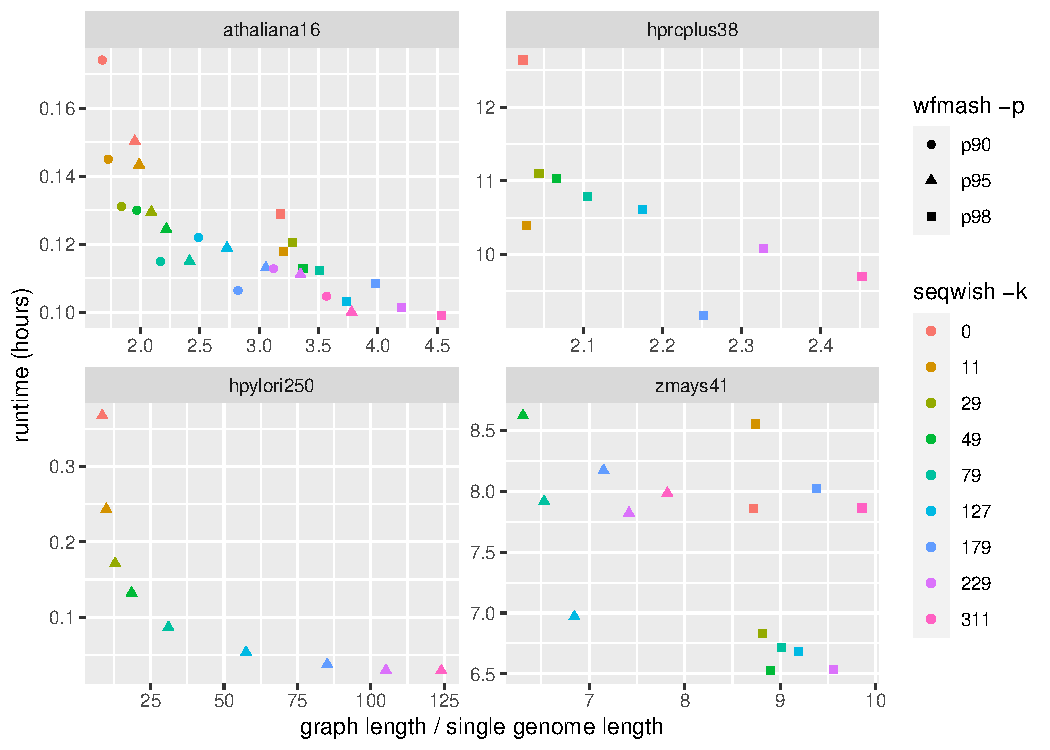
\includegraphics[width=\linewidth]{fig_experiment_stats.pdf}
   \caption{
     Experimental results from the application of \textit{seqwish} to four different pangenomes.
     Multiple minimum identity settings for the mapping (\textit{wfmash -p}) and different minimum match length filter settings result in a collection of graph builds per pangenome input.
     We compare the runtime in hours with the size of the resulting graphs relative to the average size of an input genome in the particular set.
     Lower limits on pairwise identity result in more compact graphs.
     Similarly, filtering short matches increases graph size relative to not (\textit{seqwish -k}=0, red).
     Increasing the \textit{seqwish -k} parameter tends to increase the size of the graph.
    }
    \label{fig:experiments}
\end{figure}

